\documentclass{beamer}
\usepackage[english, russian]{babel}
\usepackage[T2A]{fontenc}
\usepackage[utf8]{inputenc}
\usepackage{indentfirst}
\usepackage{amsmath, amsfonts, amssymb, amsthm, mathtools}
\usepackage[export]{adjustbox}
\usepackage{graphicx} 
\graphicspath{ {./images/} }

\usepackage{subcaption}
\usepackage{verbatim}

\usepackage{minted}{\setlength{\parskip}{0pt}}

\usepackage{hyperref}

\hypersetup{
    colorlinks=true,
    linkcolor=blue,
    filecolor=magenta,      
    urlcolor=black,
    pdftitle={Overleaf Example},
    pdfpagemode=FullScreen,
    }


\title{Отчет по лабораторной работе № 15. \\ Настройка сетевого журналирования}
\author{Данила Стариков \\ НПИбд-02-22}
\date{2024}

\begin{document}

\maketitle
\newpage

\tableofcontents

\newpage
\section{Цель работы}
Получение навыков по работе с журналами системных событий.
\newpage

\section{Выполнение работы}
\subsection{Настройка сервера сетевого журнала}
\begin{enumerate}

\item На сервере создали файл конфигурации сетевого хранения журналов (Рис. \ref{img:1}):
    \begin{minted}{bash}
cd /etc/rsyslog.d
touch netlog-server.conf
    \end{minted}

\begin{center}
    \centering
    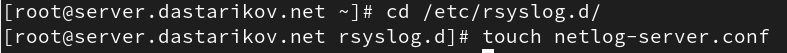
\includegraphics[width=\textwidth]{../images/image01.png}
    \captionof{figure}{Создание файла конфигурации для сетевого хранения журналов на сервере.}
    \label{img:1}
\end{center}

\item В файле конфигурации {\tt /etc/rsyslog.d/netlog-server.conf} включили приём записей журнала по TCP-порту 514 (Рис. \ref{img:2}):
    \begin{minted}{bash}
$ModLoad imtcp
$InputTCPServerRun 514
    \end{minted}

\begin{center}
    \centering
    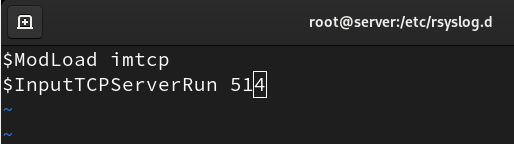
\includegraphics[width=\textwidth]{../images/image02.png}
    \captionof{figure}{Включение приема записей журнала по TCP-порту 514.}
    \label{img:2}
\end{center}

\item Перезапустили службу {\tt rsyslog} и посмотрели, какие порты, связанные с {\tt rsyslog}, прослушиваются (Рис. \ref{img:3}):
    \begin{minted}{bash}
systemctl restart rsyslog
lsof | grep TCP
    \end{minted}

\begin{center}
    \centering
    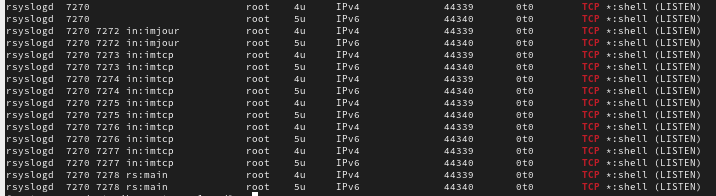
\includegraphics[width=\textwidth]{../images/image03.png}
    \captionof{figure}{Проверка прослушиваемых rsyslog портов.}
    \label{img:3}
\end{center}

\item На сервере настроили межсетевой экран для приёма сообщений по TCP-порту 514 (Рис. \ref{img:4}):
    \begin{minted}{bash}
firewall-cmd --add-port=514/tcp
firewall-cmd --add-port=514/tcp --permanent
    \end{minted}

\begin{center}
    \centering
    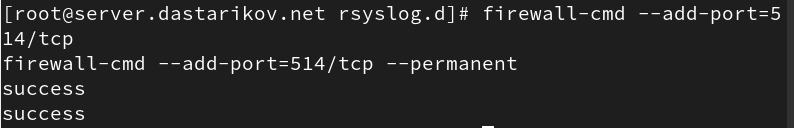
\includegraphics[width=\textwidth]{../images/image04.png}
    \captionof{figure}{Настройка межсетевого экрана для приема сообщений по TCP-порту 514.}
    \label{img:4}
\end{center}
\end{enumerate}

\subsection{Настройка клиента сетевого журнала}
\begin{enumerate}
\item На клиенте создали файл конфигурации сетевого хранения журналов (Рис. \ref{img:5}):
    \begin{minted}{bash}
cd /etc/rsyslog.d
touch netlog-client.conf
    \end{minted}

\begin{center}
    \centering
    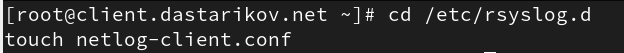
\includegraphics[width=\textwidth]{../images/image05.png}
    \captionof{figure}{Создание файла конфигурации сетевого хранения журналов на клиенте.}
    \label{img:5}
\end{center}

\item На клиенте в файле конфигурации {\tt /etc/rsyslog.d/netlog-client.conf} включили перенаправление сообщений журнала на 514 TCP-порт сервера (Рис. \ref{img:6}):
    \begin{minted}{bash}
*.* @@server.dastarikov.net:514
    \end{minted}

\begin{center}
    \centering
    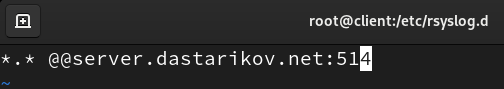
\includegraphics[width=\textwidth]{../images/image06.png}
    \captionof{figure}{Включение перенаправления сообщений журнала на сервер через TCP-порт 514.}
    \label{img:6}
\end{center}

\item Перезапустили службу {\tt rsyslog} (Рис. \ref{img:7}):
    \begin{minted}{bash}
systemctl restart rsyslog
    \end{minted}


\begin{center}
    \centering
    
\includegraphics[width=\textwidth]{../images/image07.png}
    \captionof{figure}{Перезапуск службы rsyslog.}
    \label{img:7}
\end{center}
\end{enumerate}

\subsection{Просмотр журнала}
\begin{enumerate}
\item На сервере просмотрели один из файлов журнала (Рис. \ref{img:8})
    \begin{minted}{bash}
tail -f /var/log/messages
    \end{minted}

\begin{center}
    \centering
    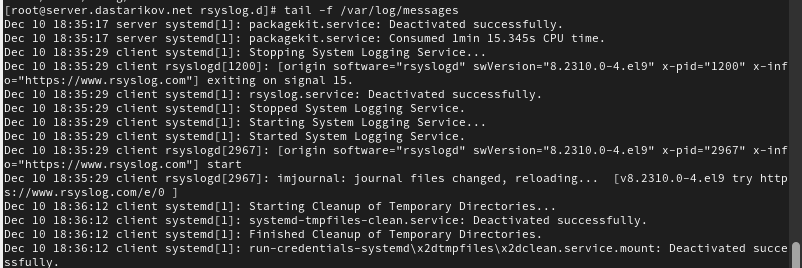
\includegraphics[width=\textwidth]{../images/image08.png}
    \captionof{figure}{Просмотр файла журнала на сервере.}
    \label{img:8}
\end{center}

Обратите внимание на имя хоста и другие сообщения о работе сервисов. При наличии сообщений о некорректной работе сервисов исправьте ошибки в настройках соответствующих служб.

\item На сервере под пользователем dastarikov запустили графическую программу для просмотра журналов (Рис. \ref{img:9}):
    \begin{minted}{bash}
gnome-system-monitor
    \end{minted}

\begin{center}
    \centering
    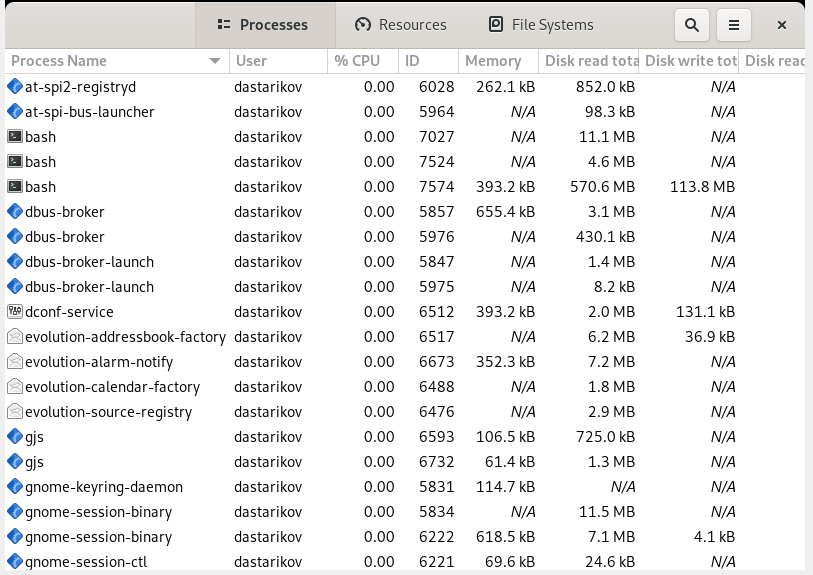
\includegraphics[width=\textwidth]{../images/image09.png}
    \captionof{figure}{Просмотр журнала на клиенте через графическую программу.}
    \label{img:9}
\end{center}

\item На сервере установили просмотрщик журналов системных сообщений {\tt lnav} или его аналог (Рис. \ref{img:10}):
    \begin{minted}{bash}
dnf -y install lnav
    \end{minted}

\begin{center}
    \centering
    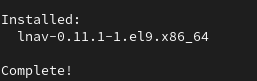
\includegraphics[width=\textwidth]{../images/image10.png}
    \captionof{figure}{Установка просмотрщика журналов системных сообщений на сервер.}
    \label{img:10}
\end{center}

\item Просмотрели логи с помощью {\tt lnav} (Рис. \ref{img:11} и \ref{img:11a}):
    \begin{minted}{bash}
lnav
    \end{minted}

\begin{center}
    \centering
    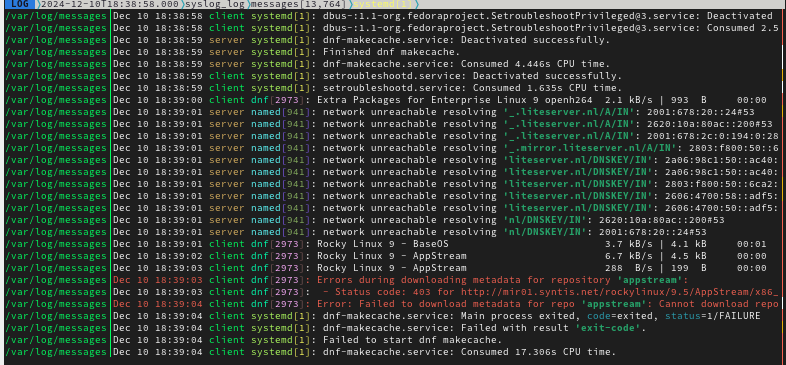
\includegraphics[width=\textwidth]{../images/image11.png}
    \captionof{figure}{Просмотр общих логов на сервере.}
    \label{img:11}
\end{center}

\begin{center}
    \centering
    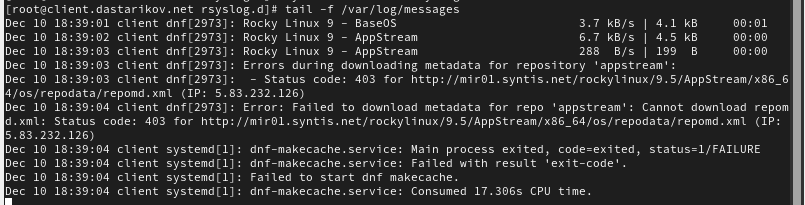
\includegraphics[width=\textwidth]{../images/image11a.png}
    \captionof{figure}{Логи на клиенте.}
    \label{img:11a}
\end{center}

Можно заметить, что все логи, имеющиеся на клиенте, также присутствуют и на сервере соответствующей отметкой о принадлежности.
\end{enumerate}

\subsection{Внесение изменений в настройки внутреннего окружения виртуальных машин}
\begin{enumerate}
\item На виртуальной машине {\tt server} перешли в каталог для внесения изменений в настройки внутреннего окружения {\tt /vagrant/provision/server/}, создали в нём каталог {\tt netlog}, в который поместили в соответствующие подкаталоги конфигурационные файлы (Рис. \ref{img:12}):
    \begin{minted}{bash}
cd /vagrant/provision/server
mkdir -p /vagrant/provision/server/netlog/etc/rsyslog.d
cp -R /etc/rsyslog.d/netlog-server.conf /vagrant/provision/server/netlog/etc/rsyslog.d
    \end{minted}
\item В каталоге {\tt /vagrant/provision/server} создали исполняемый файл {\tt netlog.sh} (Рис. \ref{img:12}):
    \begin{minted}{bash}
cd /vagrant/provision/server
touch netlog.sh
chmod +x netlog.sh
    \end{minted}

\begin{center}
    \centering
    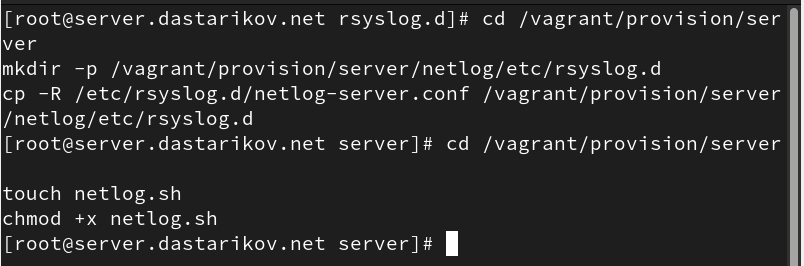
\includegraphics[width=\textwidth]{../images/image12.png}
    \captionof{figure}{Создание каталога для настройки внутреннего окружения на сервере.}
    \label{img:12}
\end{center}

Открыли его на редактирование, прописали в нём следующий скрипт:
    \begin{minted}{bash}
#!/bin/bash
echo "Provisioning script $0"
echo "Copy configuration files"
cp -R /vagrant/provision/server/netlog/etc/* /etc
restorecon -vR /etc
echo "Configure firewall"
firewall-cmd --add-port=514/tcp
firewall-cmd --add-port=514/tcp --permanent
echo "Start rsyslog service"
systemctl restart rsyslog
    \end{minted}
\item На виртуальной машине {\tt client} перешли в каталог для внесения изменений в настройки внутреннего окружения {\tt /vagrant/provision/client/}, создали в нём каталог {\tt nentlog}, в который поместили в соответствующие подкаталоги конфигурационные файлы (Рис. \ref{img:13}):
    \begin{minted}{bash}
cd /vagrant/provision/client
mkdir -p /vagrant/provision/client/netlog/etc/rsyslog.d
cp -R /etc/rsyslog.d/netlog-client.conf /vagrant/provision/client/netlog/etc/rsyslog.d/
    \end{minted}
\item В каталоге {\tt /vagrant/provision/client} создали исполняемый файл {\tt netlog.sh} (Рис. \ref{img:13}):
    \begin{minted}{bash}
cd /vagrant/provision/client
touch netlog.sh
chmod +x netlog.sh
    \end{minted}

\begin{center}
    \centering
    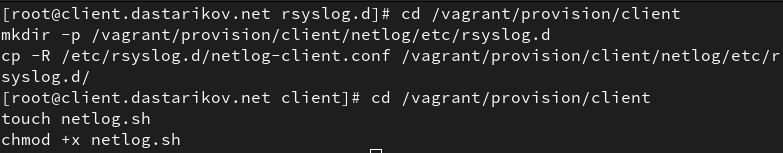
\includegraphics[width=\textwidth]{../images/image13.png}
    \captionof{figure}{Создание каталога для настройки внутреннего окружения на клиенте.}
    \label{img:13}
\end{center}

Открыв его на редактирование, прописали в нём следующий скрипт:
    \begin{minted}{bash}
#!/bin/bash
echo "Provisioning script $0"
echo "Install needed packages"
dnf -y install lnav
echo "Copy configuration files"
cp -R /vagrant/provision/client/netlog/etc/* /etc
restorecon -vR /etc
echo
systemctl restart rsyslog
    \end{minted}
\item Для отработки созданных скриптов во время загрузки виртуальных машин {\tt server} и {\tt client} в конфигурационном файле {\tt Vagrantfile} добавили в соответствующих разделах конфигураций для сервера и клиента:
    \begin{minted}{bash}
server.vm.provision "server netlog",
type: "shell",
preserve_order: true,
path: "provision/server/netlog.sh"
client.vm.provision "client netlog",
type: "shell",
preserve_order: true,
path: "provision/client/netlog.sh"
    \end{minted}

\end{enumerate}


\section{Выводы}
В результате выполнений лабораторной работы получили навыки настройки сетевого хранения журналов системных событий.

\end{document}
